
\textbf{Shared Memory:} 
Because multithreaded programs frequently use updates to shared memory to communicate, \dthreads{} must implement a mechanism to expose one thread's updates to all other threads.  At the beginning of a transaction, all shared pages are protected, and can only be read by threads.  When a thread attempts to modify a shared page a local working copy is created, leaving the shared page unmodified.  At commit time, a ``twin'' copy of all modified pages is created.  Every page is compared to its twin (using a byte-wise diff) and modified bytes are copied back to the shared state.  Unlike transactional memory, conflicting changes do not result in rollbacks with \dthreads{}.  Further details are described in Section~\ref{sec:sharedmemory}.


\section{\dthreads{} Architecture}
\label{sec:dthreads-architecture}
This section describes \dthreads{}’ key algorithms—memory isolation, deterministic (diff-based) memory commit, deterministic synchronization, and deterministic memory allocation—as well as other implementation details.

\subsection{Isolated Memory Access}
\label{sec:threadsasprocs}

In order to achieve the deterministic memory access, 
\dthreads{} isolates memory accesses among different
threads between commit points, and commits the updates of each thread deterministically.

To isolate the memory access among different threads, \dthreads{} are treating threads as processes.  In a multi-threading program running with \pthreads{}, threads share all memory except for the stack.  Changes to memory are immediately visible to all other threads.  Threads share the same file descriptors, sockets, device handles, and windows. Because \dthreads{} runs threads in separate processes, these shared resources must be explicitly managed by the runtime library.

\subsubsection{Thread Creation}
\dthreads{} interposes those \texttt{pthread\_create()} functions and replaces them with \texttt{clone} system calls. By using  \texttt{CLONE\_FILES} flag, \dthreads{} create processes that have distinct address space but share the same file descriptor table. Also, \dthreads{} shims the \texttt{getpid()} function to return a single, globally-shared process identifier. 

\subsubsection{Deterministic Thread Index}
\label{sec:threadindex}

POSIX does not guarantee deterministic process or thread identifiers. To avoid exposing this nondeterminism to threads running as processes, \dthreads{} shims the \texttt{pthread\_self()} function in order to return an internal thread index.  This internal thread index is managed using a single global variable that is incremented on thread creation.  This unique thread index is also used to manage per-thread heaps and as an offset into an array of thread entries.

\subsubsection{Shared Memory}
\label{sec:stackandheap}

In order to create the illusion that different threads are sharing the same address space, \dthreads{} uses memory mapped files to share the globals and heap across different processes(globals and heap, but not heap, see Section~\ref{sec:discussion}).

\dthreads{} creates two different mappings for both the heap and the globals.  One is a shared mapping, which is used to hold shared state. The other is a private, copy-on-write (COW) per-process mapping that each process works on directly.  Private mappings are linked to the shared mapping through the single fixed-size memory mapped file. Reads initially go directly to the shared mapping,
but after the first write operation, both reads and writes are entirely private.

Memory allocations are issued from the shared heap memory using a scalable per-thread heap organization loosely based on Hoard~\cite{BergerMcKinleyBlumofeWilson:ASPLOS2000} and built using HeapLayers~\cite{BergerZornMcKinley:2001}.  \dthreads{} divides the heap into a fixed number of sub-heaps (currently 16).  Each thread uses a hash of its thread index to find the appropriate sub-heap.

\subsection{Deterministic Memory Commit}
\label{sec:sharedmem}

\begin{figure}
{\centering 
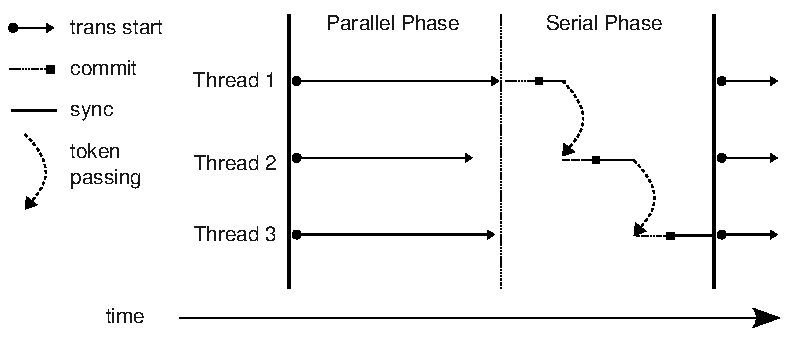
\includegraphics[width=3.25in]{dthreads/figure/phase}
\caption{An overview of \dthreads{} phase. Program execution with \dthreads{} alternates between parallel and serial phases.\label{fig:phase}}
}
\end{figure}

Figure~\ref{fig:phase} illustrates the execution of programs under \dthreads{}.  To guarantee determinism, \dthreads{} isolates memory accesses in parallel phases. In parallel phases, memory accesses work on private copies after the first write operation and updates are not shared across threads.  When a synchronization point is reached, updates are exposed in deterministic order.  This section describes the mechanisms used to guarantee deterministic commit order, and the details of commits to shared memory.

\subsubsection{Fence and Token}
\label{sec:schedule}

\dthreads{} places internal fences between the parallel and serial phases. \dthreads{} re-implements the fence because the standard \pthreads{} barrier mechanism does not support dynamic changes of threads number. 

\begin{figure}
\begin{lstlisting} [style=tt]
void waitFence(void) {
  lock();
	
  while(!isArrivalPhase()) { 
    CondWait();
  }

  waiting_threads++;
  if(waiting_threads < alive_threads) {
    while(!isDeparturePhase()) {
      CondWait();
    }
  } 
  else {
    setDeparturePhase();
    CondBroadcast();
  }

  waiting_threads--;
  if (waiting_threads == 0) {
    setArrivalPhase();
    CondBroadcast();
  }

  unlock();
}

\end{lstlisting}
\caption{Pseudocode for the internal fence.\label{fig:internalFence}}
\end{figure}

Figure~\ref{fig:internalFence} shows the pseudocode code for the internal fence. Threads must wait at the fence 
until all threads from the previous fence have departed. Then those threads are waiting on the fence until all alive threads  have entered into the same fence(lines 8-11). 
The last thread entering the fence initiates the departure phase and wakes up all threads on the fence(lines 14-15). As threads leave the fence, they decrement the waiting thread count.  The last thread to leave sets the fence to the arrival phase and wakes any waiting threads (lines 19-21).

To reduce overhead, whenever the number of running threads is
less than or equal to the number of cores, waiting threads block by spinning rather than by invoking relatively expensive cross-process \pthreads{} mutexes. When the number of threads exceeds the number of cores, \dthreads{} falls back to using \pthreads{} mutexes.

\begin{figure}
\begin{lstlisting} [style=tt]
void waitToken() {
  waitFence();
  while(isNotMyToken()) { yield(); }
}
void putToken() {
  passTokenToNextOfTokenQueue();
}
\end{lstlisting}
\caption{Pseudocode for waitToken and putToken. 
\label{fig:token}}
\end{figure}

Another key mechanism of \dthreads{} is using the token to order memory commits and synchronizations. The token implementation is listed in Figure~\ref{fig:token}. The token is a shared pointer that points to the next runnable thread entry, which guarantees the global order for all operations in serial phases.  

\dthreads{} introduces two subroutines to manage tokens.  The\texttt{waitToken()} function first waits at the internal fence and then waits to acquire the global token
in order to enter serial mode. The \texttt{putToken()} function passes the token to the next waiting thread. 

As shown in Figure~\ref{fig:phase}, it is very important for a thread to wait at the internal fence before a thread enters into serial phases or before a thread leaves serial phases, even for a thread that is guaranteed to have the token next. Memory commits by a thread can affect other threads' behavior. 

\subsubsection{Commit Protocol}
\begin{figure}
{\centering
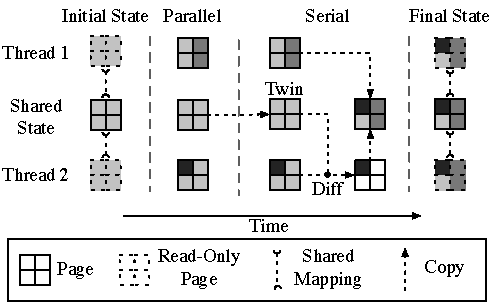
\includegraphics[width=5in]{dthreads/figure/architecture-diagram}
\caption{An overview of \dthreads{} execution.\label{fig:architecture}}
}
\end{figure}

Figure~\ref{fig:architecture} shows the steps to capture modifications to shared state and expose them in a deterministic order.  

At the beginning of the parallel phases, different threads have a read-only mapping for all shared pages. If a thread writes to a shared page during the parallel phases, this write is trapped in order to create a private copy and a twin page for this shared page. After that, reads and writes on this page happen on the private copy only. Reads go directly to the shared memory and are not trapped.  

In the serial phases, threads first commit their local changes happening in parallel phases one at a time, guided by the global token.  The first thread to commit to a page can directly copy its private copy to the shared state, but subsequent commits must copy only the modified bytes. To find out those modifications, \dthreads{} compares those private copies against those twin pages, creating from the shared mapping before actual modification.  After a thread commits its local changes, it issues synchronizations before it passes the token to next thread. 

In the end of serial phase, every threads have to wait at the fence in order to enter into the next parallel phase. 

\subsection{Deterministic Synchronization}
\label{sec:synchronization}
\dthreads{} supports the full range of synchronizations of
\pthreads{} APIs, including locks, conditional variables, barriers and different types of thread exit.

\subsubsection{Locks}
\dthreads{} uses the global token to guide synchronizations during the serial phases. Before a thread is acquiring a lock while current thread does not have the token, it has to wait for the global token. 

\dthreads{} treats multiple locks as the same one, which  possibly compromise the efficiency of programs, it only ends the serial phases when all locks are unlocked. Thus, it is possible for a program with deadlock problems that those deadlock do not occur to \dthreads{} at all. 

For the acquisitions of locks, \dthreads{} checks at first 
whether the current thread is already holding any locks. If not, the thread first waits for the token, commits those changes happened in the last parallel phase to shared state, and begins a new atomic section. Finally, the thread increments the number of locks it is currently holding. The lock count ensures that a thread does not pass the token to the next one until it has released all of the locks.

During the releases of locks, \dthreads{} decrements the lock count at first. A thread does nothing if there are still some locks holding by the current thread, with the lock count not equal to 0. If all locks have been released, \dthreads{} commits the memory changes happened in this serial phase to the shared mapping. Then it passes the global token to the next thread of the token queue and starts a new atomic region. Finally, the thread waits on the internal fence before enter inginto the next round's parallel phase.

\subsubsection{Condition Variables}
\label{sec:condwait}

Guaranteeing determinism for condition variables is much more complex than for other synchronization operations. The underlying operating system can not guarantee that threads are going to be waken-up in the same order as they wait on a conditional variable. Thus, a naive implementation easily leads to a deadlock problem.

//NOW
Different with the busy wait mechanism that CoreDet used, 
\dthreads{} tries to reduce the performance cost
introduced by busy wait mechanism. Since we have no idea when those
waiting threads will be awakened, we don't want those threads to be
checked frequently since this can cause expensive process
switches. Also, we don't want those waiting threads to thwart the the
token passing of non-waiting threads.
In \dthreads{}, waiting threads are extracted from the normal run
queue and inserted into the corresponding queue of condition
variable so that the token will not be passed to these waiting
threads.

By inserting threads into corresponding queue of condition
variables, which can help those signal and broadcast function to find
out which thread should be waken up firstly and to avoid the
un-determinism brought by operating system. We enforce the
first-in-first-out rule for all waiting threads.

Since those threads calling \texttt{cond\_wait} should get the token in order
to ensure the determinism, they have to release the token to next
thread in the active list. After finishing these work, then those
threads can actually wait on the real process-shared conditional
variable.

After one thread is awakened, the thread should try to get token at
first in order to proceed since the thread being awakened is 
still inside the critical section (under lock protection)
and the token is required to guarantee determinism under the critical region. 

\dthreads{} uses the busy wait mechanism to get the global token. 
It is noted that this new awakened thread don't need to call \texttt{waitToken()} to get
token since \texttt{waitToken()} should wait for all alive threads to reach the fence at first. 
Now the waking thread has already passed the fence, calling \texttt{waitToken()} can potentially
put this new awakened thread to the next run of serial phase, which not only hurts
the performance but also introduce some possible deadlock.

\begin{figure}
\begin{lstlisting}
void cond_wait (pthread_cond_t * cond) {
  waitToken();
  atomicEnd(false);
  removeFromTokenQueue();
  insertToTailOfCondqueue();
  decreaseInternalFence();
  putToken();
  // Only proceed if I am ready to run.
  while (!isReadyToGo()) { real_condwait(); }
  while (isNotMyToken()) { yield(); } 
  atomicBegin();
  // Token can be released in unlock. 
}
\end{lstlisting}
\caption{Pseudocode for \texttt{cond\_wait} ($\S$~\ref{sec:condwait}). 
\label{fig:condwait}}
\end{figure}

Figure~\ref{fig:condwait} presents pseudocode
for \texttt{cond\_wait}.  When a thread executes \texttt{cond\_wait},
it first awaits the token (line 2) before it can proceed.  It then
commits local modifications, removes itself from the token queue, and
places itself at the tail of conditional variable's queue (lines
3--5). It then decreases the internal fence thread count (line 6) and passes
the token to the next entry on the token queue (line 7). When a thread
is awakened by a signal, it checks whether the current thread is in
fact ready to run (line 9), since multiple threads can be awakened
by \texttt{cond\_signal} but only the first thread can run.  Finally,
it waits for the token to enter into the serial phase (line 12). 

\label{sec:condsignal}

\begin{figure}
\begin{lstlisting}
void cond_signal() {
  if(!isHoldingToken())
    waitToken();
  atomicEnd(false);
  if(noWaiters()) return;
  lock();
  thread = getFirstThreadOfCondQueue();
  insertToHeadOfTokenQueue();
  setThreadReadyToGo();
  incrementInternalFence();
  unlock();
  atomicBegin();
}
\end{lstlisting}
\caption{Pseudocode for \texttt{cond\_signal} ($\S$~\ref{sec:condsignal}). 
\label{fig:condsignal}}
\end{figure}

In \pthreads{}, the only difference between \texttt{cond\_signal}
and \texttt{cond\_broadcast} is that \texttt{cond\_signal} only wakes up the
first thread, while \texttt{cond\_broadcast} wakes up all threads in the
queue. To guarantee determinism for \texttt{cond\_signal}, \dthreads{}
broadcasts the signal to all threads blocked on the condition
variable, but only the status of first thead in the queue can be set
to runnable, so other threads will have to wait on the condition
variable again (see~\ref{fig:condwait}).
These functions remove the corresponding threads from the queue
of condition variable and insert them to the header of active list,
thus those threads can get token next.  Note that it is very important
to do so both to avoid deadlock and to improve performance. By placing
awakened threads on the next runnable position rather than on the tail
of the run queue, \dthreads{} avoids possible deadlocks. 
Thus, these awakened threads can run immediately (see line 10 of Figure~\ref{fig:condwait}) 
after getting the token, which improves performance. Finally, the
signaling thread releases the token to awakened threads.

Figure~\ref{fig:condsignal} presents the pseudocode
for \texttt{cond\_signal}. Before proceeding, the caller waits for
the token if it is not holding it already, and commits any local
modifications (lines 2--4).  If there are no waiters on the
conditional variable, it returns immediately. Otherwise, \dthreads{}
removes the first thread from the condvar's queue and places it at the
head of the token queue (lines 7--8). Finally, it makes this thread
runnable and increase the internal fence's thread count (line 9--10).

\subsubsection{Barriers}

\label{sec:barrierwait}

\begin{figure}
\begin{lstlisting}
void barrier_wait() {
  waitToken(); atomicEnd(false);
 
  lock();
  if(isLastThreadEnterBarrier()) {
	moveWholelistBacktoTokenqueue();
	increaseInternalFence(waitersNumb);
	passTokenToFirstOfBarrQueue();
  } 
  else {
    removeFromTokenqueue();
	insertTailOfBarrQueue();
	putToken();
  }
  unlock();

  atomicBegin();
  realBarrierWait();  
}
\end{lstlisting}
\caption{Pseudocode for barrier\_wait ($\S$~\ref{sec:barrierwait}).
\label{fig:barrierwait}}
\end{figure}

As with condition variables, \dthreads{} must ensure that threads
waiting on a barrier do not disrupt the token passing of running
threads. \dthreads{} removes threads entering into the barrier from
the run queue and places them on the corresponding barrier queue.

To avoid blocking on the barrier, the last thread entering into
the barrier moves all threads to the runnable queue and increases
the fence's thread count.

Figure~\ref{fig:barrierwait} presents pseudocode
for \texttt{barrier\_wait}. The calling thread first waits for the
token to commit any local modifications in order to ensure
deterministic commit (lines 2 and 3). If the current thread is the
last to enter the barrier, then \dthreads{} moves the entire list of
threads on the barrier queue to the token queue (line 7), increases
the fence's thread count (line 8), and passes the token to the first thread in the
barrier queue (line 9).  Otherwise, \dthreads{} removes the current
thread from the token queue (line 12), places it on the barrier queue
(line 13), and releases token (line 14). Finally, the thread waits on
the actual barrier (line 19).

\subsubsection{Thread Creation and Exit}

\label{sec:threadcreation}

\begin{figure}
\begin{lstlisting}
void thread_create () {
  waitToken();
  clone(CLONE_FS| CLONE_FILES | CLONE_CHILD);
  if(isChild) {
    getGlobalThreadIndex();
	insertToTokenQueue();
	notifyChildRegistered();
	// Await notification until parent reaches 
    // next sync point after spawning.
	waitParentBroadcast();	
  }
  else if (isParent) {
	waitChildRegistered();
  }
}
\end{lstlisting}
\begin{lstlisting}
void thread_exit() {
  waitToken();
  atomicEnd(false);
  removeFromTokenQueue();
  decreaseInternalFence();
  putToken();
  exitThread(); 
}
\end{lstlisting}
\caption{Pseudocode for thread creation and exit ($\S$~\ref{sec:threadcreation}).
\label{fig:threadcreation}
}
\end{figure}

To guarantee determinism, thread creation and exit must be performed in the serial phase.  Newly created threads are immediately added to the token queue.  Creating a thread does not immediately release the token; this allows a single thread to quickly create multiple child threads without waiting for a new serial phase for each.

Figure~\ref{fig:threadcreation} shows pseudocode for thread creation. The caller first waits for the token before proceeding (line 2).  It then creates a new process with shared file descriptors but a distinct address space using the \texttt{clone} system call (line 3).  The newly created child obtains the global thread index (line 5), places itself in the token queue (line 6), and notifies the parent that child has registered itself in the active list (line 7). The child thread then waits for the parent to reach a synchronization point.

When \texttt{thread\_exit()} is called, the caller first waits for the token and then commits any local modifications (line 3). It then removes itself from the token queue (line 4) and decreases the number of threads required to proceed to the next phase (line 5). Finally, the thread passes its token to the next thread in the token queue (line 6) and exits (line 7).

\subsubsection{Thread Cancellation}

\dthreads{} provides the following mechanism to support
deterministic thread cancellation. First, thread cancellation can only
happen in the serial mode withholding the token, which guarantees that
only current thread trying to issue cancellation request is
running. Other threads are either waiting on condition variables or
barriers. Second, thread entry should have enough information about
their status, which can be recorded. If one thread being cancelled are
waiting on condition variable or barrier, it should be removed from
corresponding queue in order to guarantee the correctness.


\section{Optimizations}
\dthreads{} performs a number of optimizations to improve performance.

\textbf{Single Thread Case: }
When only one thread is running, \dthreads{} does not employ memory protection 
and treats all synchronization operations as no-ops.
In addition, when only one thread is active because other threads are waiting on conditional variables, 
\dthreads{} does not try to commit local changes to the shared mapping (or discard  
private dirty pages). Updates are only committed when the thread issues
a \texttt{cond\_signal} or \texttt{cond\_broadcast} call, which
will wake up a thread and thus require publication of any updates.

\textbf{Lazy Twin Creation: }
Twin pages are only created when a page has multiple writers during the same transaction.  
During the commit phase, the single writer can directly copy its working copy to the shared state 
without performing a diff. This reduces the overhead in the common case, 
where a single thread is the exclusive writer of a page.

\textbf{Commit Optimization: }
If one thread is the only writer on one page, or if it is the first thread to commit a page,
they can directly copy its working copy to shared state.
\dthreads{} currently relies on the comparison between local version number and the global page version number. 
In the page handler, each thread obtains the version number for every dirty page. 
In the commit phase, \dthreads{} compares this local version number with the global version
number to check whether it is the first writer (see Figure~\ref{fig:atomicend}).

\textbf{Parallelization: }
\dthreads{} attempts to exploit as much parallelism as possible in the runtime system itself.
For example, \texttt{atomicBegin} must perform certain bookkeeping
tasks, including releasing private page frames or resetting pages to
read-only mode.  \texttt{atomicEnd} in lock operations (see
Figure~\ref{fig:lock} not only commits, but also launders those dirty
pages modified by earlier threads.  Clearly, it is safe to cleanup all
dirty pages but that can cause a performance degradation since this
occurs in the serial phase.  By calling \texttt{atomicEnd()} with the
argument \texttt{true}, only those pages modified by earlier threads
will be cleaned up, in order to give one complete image of one page
which later transactions may refer to.
